% -*- mode: noweb; noweb-default-code-mode: R-mode; -*-
%
% Copyright (C) 2009 Markus Gesmann


\documentclass[a4paper]{article}
\usepackage{amsmath,color,hyperref}
\usepackage[round]{natbib}
\usepackage[T1]{fontenc}
\usepackage[utf8]{inputenc}
\usepackage[english]{babel}
\usepackage{Sweave}


% \VignetteIndexEntry{An R Package for claims reserving }
% \VignetteDepends{Hmisc, lattice}
% \VignetteKeyword{ChainLadder}

\newcommand{\proglang}[1]{\textsf{#1}}
\newcommand{\pkg}[1]{\textbf{#1}}
\renewcommand{\familydefault}{\sfdefault}

\bibliographystyle{plainnat}

\title{The \pkg{ChainLadder} package }
\author{Markus Gesmann\\
  markus.gesmann@gmail.com}


\begin{document}

\maketitle

\begin{abstract}
The \pkg{ChainLadder} package~\citep{chainladder} started its life out of presentations the author gave on stochastic reserving at the Institute of Actuaries from 2007 - 2009. Currently the Mack-, Munich- and Bootstrap-chain-ladder methods are implemented. The package also provides an example spreadsheet, which shows how to use the \pkg{ChainLadder} functions within Excel using the RExcel Add-in~\citep{rexcel}.
\end{abstract}
\subsection*{Thanks}
\input{"../../../THANKS"}
\clearpage
\tableofcontents
\clearpage
\section{Introduction}

\subsection{Claims reserving in insurance}
Insurance companies are different.\\[2mm]
Unlike any other industry insurers don't know the production cost of their product. 
Insurers sell the promise to pay for future claims occurring over an agreed period for an
upfront received premium. The estimated future claim payments have to be held
in the reserves, one of the biggest liability items on an insurer's balance sheet.
The \pkg{ChainLadder} package can help to assess those reserves.

\subsection{Typical scenario}
Usually an insurance portfolio is split into ''homogeneous" classes of business,
e.g. motor, marine, property, etc. Policy claims data are than aggregated by class of business, origin- and development period. This cross-tab view of historical claims developments looks in most cases like a triangle, filled with figures in in the top left area. The objective is to forecast future claims developments, which would fill the bottom right of the matrix, see Figure~\ref{triangle}. The difference between the estimated ultimate claims costs and claims paid to date have to be held in the reserves.
\begin{figure}[h]
  \begin{center}
    \includegraphics[width=0.4\textwidth]{Triangles}
    \caption{Schematic example of a claims triangles}\label{triangle}
  \end{center}
\end{figure}

\subsection{Stochastic reserving }
Over recent years stochastic methods have been developed and published, to provide more information than just a point estimator of the reserves. Changes in regulatory requirements such as Solvency II will foster the usage of stochastic reserving methods.
However, their usage seems to be inhibited by the usage of Excel as the standard tool for reserve analysis, which  is not an ideal environment for implementing those stochastic methods.
Our idea is to use R to implement stochastic reserving
methods, and to share them in the \pkg{ChainLadder} package via CRAN.
Using R as a language of choice gives us also the opportunity to embed the developed R functions back into Excel via the RExcel Addin~\cite{rexcel}. Therefore colleagues who are afraid of R can continue to use Excel as a front end. The \pkg{ChainLadder} package provides a spreadsheet showing some basic examples. The following R command \texttt{system.file("Excel", package="ChainLadder")} will give you the details to the folder containing the Excel spreadsheet.

\subsection{Getting started}
Start R and type for
\subsubsection{Installation:}
\texttt{install.packages("ChainLadder")}
\subsubsection{Loading the package:}
\texttt{library(ChainLadder)}
\subsubsection{Help:}
\texttt{?ChainLadder}
\subsubsection{Examples:}
\texttt{example(ChainLadder)}
\subsection{Example data sets }
The ChainLadder package comes with some example data sets, e.g.
\begin{Schunk}
\begin{Sinput}
> library(ChainLadder)
\end{Sinput}
\begin{Soutput}
ChainLadder version 0.1.2-14 by Markus Gesmann <markus.gesmann@gmail.com>

Type library(help='ChainLadder') or ?ChainLadder
to see overall documentation.

Type example(ChainLadder) to get an idea of the functionality of this package.

Feel free to send me an email if you would like to keep informed of
new versions or if you have any feedback, ideas, suggestions or would
like to collaborate.

More information is available on the ChainLadder project web-site:
http://code.google.com/p/chainladder/
\end{Soutput}
\begin{Sinput}
> RAA
\end{Sinput}
\begin{Soutput}
        1     2     3     4     5     6     7     8     9    10
1981 5012  8269 10907 11805 13539 16181 18009 18608 18662 18834
1982  106  4285  5396 10666 13782 15599 15496 16169 16704    NA
1983 3410  8992 13873 16141 18735 22214 22863 23466    NA    NA
1984 5655 11555 15766 21266 23425 26083 27067    NA    NA    NA
1985 1092  9565 15836 22169 25955 26180    NA    NA    NA    NA
1986 1513  6445 11702 12935 15852    NA    NA    NA    NA    NA
1987  557  4020 10946 12314    NA    NA    NA    NA    NA    NA
1988 1351  6947 13112    NA    NA    NA    NA    NA    NA    NA
1989 3133  5395    NA    NA    NA    NA    NA    NA    NA    NA
1990 2063    NA    NA    NA    NA    NA    NA    NA    NA    NA
\end{Soutput}
\end{Schunk}
\begin{figure}[h]
  \begin{center}
\begin{Schunk}
\begin{Soutput}
NULL
\end{Soutput}
\end{Schunk}
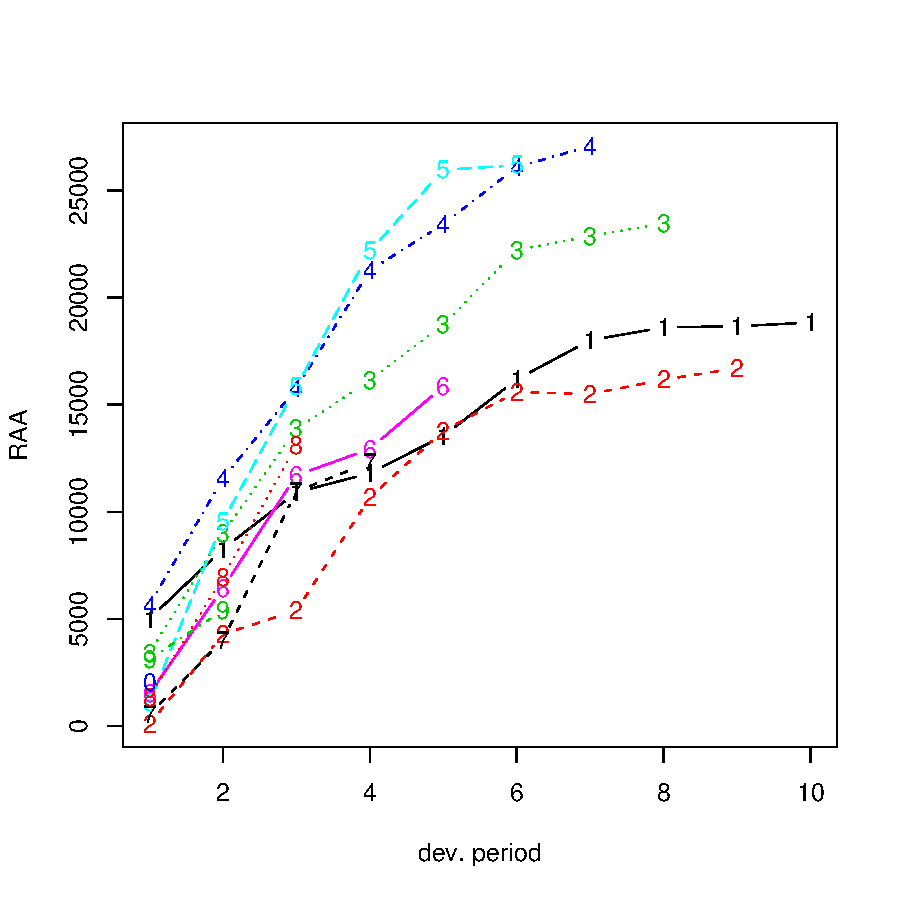
\includegraphics{ChainLadder-002}
    \caption{\texttt{plot(RAA)}}
  \end{center}
\end{figure}

\subsection{Working with triangles}
Most reserving methods are applied on data stored in a triangle format, usually with origin periods in rows and development periods in columns. However, claims development should be stored in table like formats in databases.

Also one distinguish between cumulative and incremental claims development pattern.
Transform from cumulative to incremental
\begin{Schunk}
\begin{Sinput}
> incRAA <- cbind(RAA[, 1], t(apply(RAA, 1, diff)))
> incRAA
\end{Sinput}
\begin{Soutput}
             2    3    4    5    6    7   8   9  10
1981 5012 3257 2638  898 1734 2642 1828 599  54 172
1982  106 4179 1111 5270 3116 1817 -103 673 535  NA
1983 3410 5582 4881 2268 2594 3479  649 603  NA  NA
1984 5655 5900 4211 5500 2159 2658  984  NA  NA  NA
1985 1092 8473 6271 6333 3786  225   NA  NA  NA  NA
1986 1513 4932 5257 1233 2917   NA   NA  NA  NA  NA
1987  557 3463 6926 1368   NA   NA   NA  NA  NA  NA
1988 1351 5596 6165   NA   NA   NA   NA  NA  NA  NA
1989 3133 2262   NA   NA   NA   NA   NA  NA  NA  NA
1990 2063   NA   NA   NA   NA   NA   NA  NA  NA  NA
\end{Soutput}
\end{Schunk}
Transform from incremental to cumulative
\begin{Schunk}
\begin{Sinput}
> cumRAA <- t(apply(incRAA, 1, cumsum))
\end{Sinput}
\end{Schunk}
Triangles to long format
\begin{Schunk}
\begin{Sinput}
> lRAA <- expand.grid(origin = as.numeric(dimnames(RAA)$origin), 
+     dev = as.numeric(dimnames(RAA)$dev))
> lRAA$value <- as.vector(RAA)
> head(lRAA)
\end{Sinput}
\begin{Soutput}
  origin dev value
1   1981   1  5012
2   1982   1   106
3   1983   1  3410
4   1984   1  5655
5   1985   1  1092
6   1986   1  1513
\end{Soutput}
\end{Schunk}
Long format to triangle (see later for as.ArrayTriangle function, works much better with ChainLadder)
\begin{Schunk}
\begin{Sinput}
> reshape(lRAA, timevar = "dev", idvar = "origin", v.names = "value", 
+     direction = "wide")
\end{Sinput}
\begin{Soutput}
   origin value.1 value.2 value.3 value.4 value.5 value.6 value.7 value.8
1    1981    5012    8269   10907   11805   13539   16181   18009   18608
2    1982     106    4285    5396   10666   13782   15599   15496   16169
3    1983    3410    8992   13873   16141   18735   22214   22863   23466
4    1984    5655   11555   15766   21266   23425   26083   27067      NA
5    1985    1092    9565   15836   22169   25955   26180      NA      NA
6    1986    1513    6445   11702   12935   15852      NA      NA      NA
7    1987     557    4020   10946   12314      NA      NA      NA      NA
8    1988    1351    6947   13112      NA      NA      NA      NA      NA
9    1989    3133    5395      NA      NA      NA      NA      NA      NA
10   1990    2063      NA      NA      NA      NA      NA      NA      NA
   value.9 value.10
1    18662    18834
2    16704       NA
3       NA       NA
4       NA       NA
5       NA       NA
6       NA       NA
7       NA       NA
8       NA       NA
9       NA       NA
10      NA       NA
\end{Soutput}
\end{Schunk}

\section{ChainLadder package philosophy}
Use the linear regression function "lm" as
much as possible and utilise its output
 The chain-ladder model for volume weighted
average link ratios is expressed as a formula:
\texttt{ y ~ x + 0, weights=1/x }
and can easily be changed
 Provide tests for the model assumptions

\subsection{Chain-ladder as linear regression }
Chain-ladder can be regarded as weighted linear
regression through the origin:
\begin{Schunk}
\begin{Sinput}
> x <- RAA[, 1]
> y <- RAA[, 2]
> model <- lm(y ~ x + 0, weights = 1/x)
> model
\end{Sinput}
\begin{Soutput}
Call:
lm(formula = y ~ x + 0, weights = 1/x)

Coefficients:
    x  
2.999  
\end{Soutput}
\end{Schunk}
Full regression output

The output shows:
model formula
chain-ladder link ratio
std. error of the link ratio
P-value
Residual std. error
\begin{Schunk}
\begin{Sinput}
> summary(model)
\end{Sinput}
\begin{Soutput}
Call:
lm(formula = y ~ x + 0, weights = 1/x)

Residuals:
   Min     1Q Median     3Q    Max 
-95.54 -71.50  49.03  99.55 385.32 

Coefficients:
  Estimate Std. Error t value Pr(>|t|)  
x    2.999      1.130   2.654   0.0291 *
---
Signif. codes:  0 '***' 0.001 '**' 0.01 '*' 0.05 '.' 0.1 ' ' 1 

Residual standard error: 167 on 8 degrees of freedom
  (1 observation deleted due to missingness)
Multiple R-squared: 0.4682,	Adjusted R-squared: 0.4017 
F-statistic: 7.043 on 1 and 8 DF,  p-value: 0.02908 
\end{Soutput}
\end{Schunk}
Idea: Create linear model for each development period
\begin{Schunk}
\begin{Sinput}
> ChainLadder <- function(tri, weights = 1/tri) {
+     n <- ncol(tri)
+     myModel <- vector("list", (n - 1))
+     for (i in c(1:(n - 1))) {
+         myModel[[i]] <- lm(y ~ x + 0, data.frame(x = tri[, i], 
+             y = tri[, i + 1]), weights = weights[, i])
+     }
+     return(myModel)
+ }
\end{Sinput}
\end{Schunk}
Accessing regression statistics
\begin{Schunk}
\begin{Sinput}
> CL <- ChainLadder(RAA)
> sapply(CL, coef)
\end{Sinput}
\begin{Soutput}
       x        x        x        x        x        x        x        x 
2.999359 1.623523 1.270888 1.171675 1.113385 1.041935 1.033264 1.016936 
       x 
1.009217 
\end{Soutput}
\begin{Sinput}
> sapply(lapply(CL, summary), "[[", "sigma")
\end{Sinput}
\begin{Soutput}
[1] 166.983470  33.294538  26.295300   7.824960  10.928818   6.389042   1.159062
[8]   2.807704        NaN
\end{Soutput}
\begin{Sinput}
> sapply(lapply(ChainLadder(RAA), summary), "[[", "r.squared")
\end{Sinput}
\begin{Soutput}
[1] 0.4681832 0.9532872 0.9704743 0.9976576 0.9959779 0.9985933 0.9999554
[8] 0.9997809 1.0000000
\end{Soutput}
\end{Schunk}
\section{The ChainLadder package}

Mack?s chain-ladder method calculates the standard error for the reserves estimates.
The method works for a cumulative triangle Cik if the following assumptions are hold:

$$\left\{ C_{i1},\ldots,C_{in}\right\}, \left\{ C_{j1},\ldots,C_{jn}\right\},\; i \neq j $$%,\; 1 \leq i \leq n$$
$$ E\left[ \frac{C_{i,k+1}}{C_{ik}} | C_{i1},C_{i2},\ldots,C_{ik} \right] = f_k$$
$$ \mbox{Var}\left( \frac{C_{i,k+1}}{C_{ik}} | C_{i1},C_{i2},\ldots,C_{ik} \right) = \frac{\sigma_k^2}{C_{ik}}$$
All accident years are independent

If these assumptions are hold, the Mack-chain-ladder-model gives an
unbiased estimator for IBNR (Incurred But Not Reported) claims.

\subsection{MackChainLadder}
Usage:\texttt{
MackChainLadder(Triangle,
    weights = 1/Triangle,
    est.sigma="log-linear",
    tail=FALSE, tail.se=NULL,
    tail.sigma=NULL)
}

Triangle: cumulative claims triangle
weights: default (1/Triangle) volume weighted CL
est.sigma: Estimator for sigman-1
tail, tail.se, tail.sigma: estimators for the tail

\begin{Schunk}
\begin{Sinput}
> library(ChainLadder)
> M <- MackChainLadder(Triangle = RAA, est.sigma = "Mack")
> M
\end{Sinput}
\begin{Soutput}
MackChainLadder(Triangle = RAA, est.sigma = "Mack")

     Latest Dev.To.Date Ultimate   IBNR Mack.S.E CV(IBNR)
1981 18,834       1.000   18,834      0        0      NaN
1982 16,704       0.991   16,858    154      206    1.339
1983 23,466       0.974   24,083    617      623    1.010
1984 27,067       0.943   28,703  1,636      747    0.457
1985 26,180       0.905   28,927  2,747    1,469    0.535
1986 15,852       0.813   19,501  3,649    2,002    0.549
1987 12,314       0.694   17,749  5,435    2,209    0.406
1988 13,112       0.546   24,019 10,907    5,358    0.491
1989  5,395       0.336   16,045 10,650    6,333    0.595
1990  2,063       0.112   18,402 16,339   24,566    1.503

               Totals
Latest:    160,987.00
Ultimate:  213,122.23
IBNR:       52,135.23
Mack S.E.:  26,909.01
CV(IBNR):        0.52
\end{Soutput}
\end{Schunk}
\begin{figure}[h]
  \begin{center}
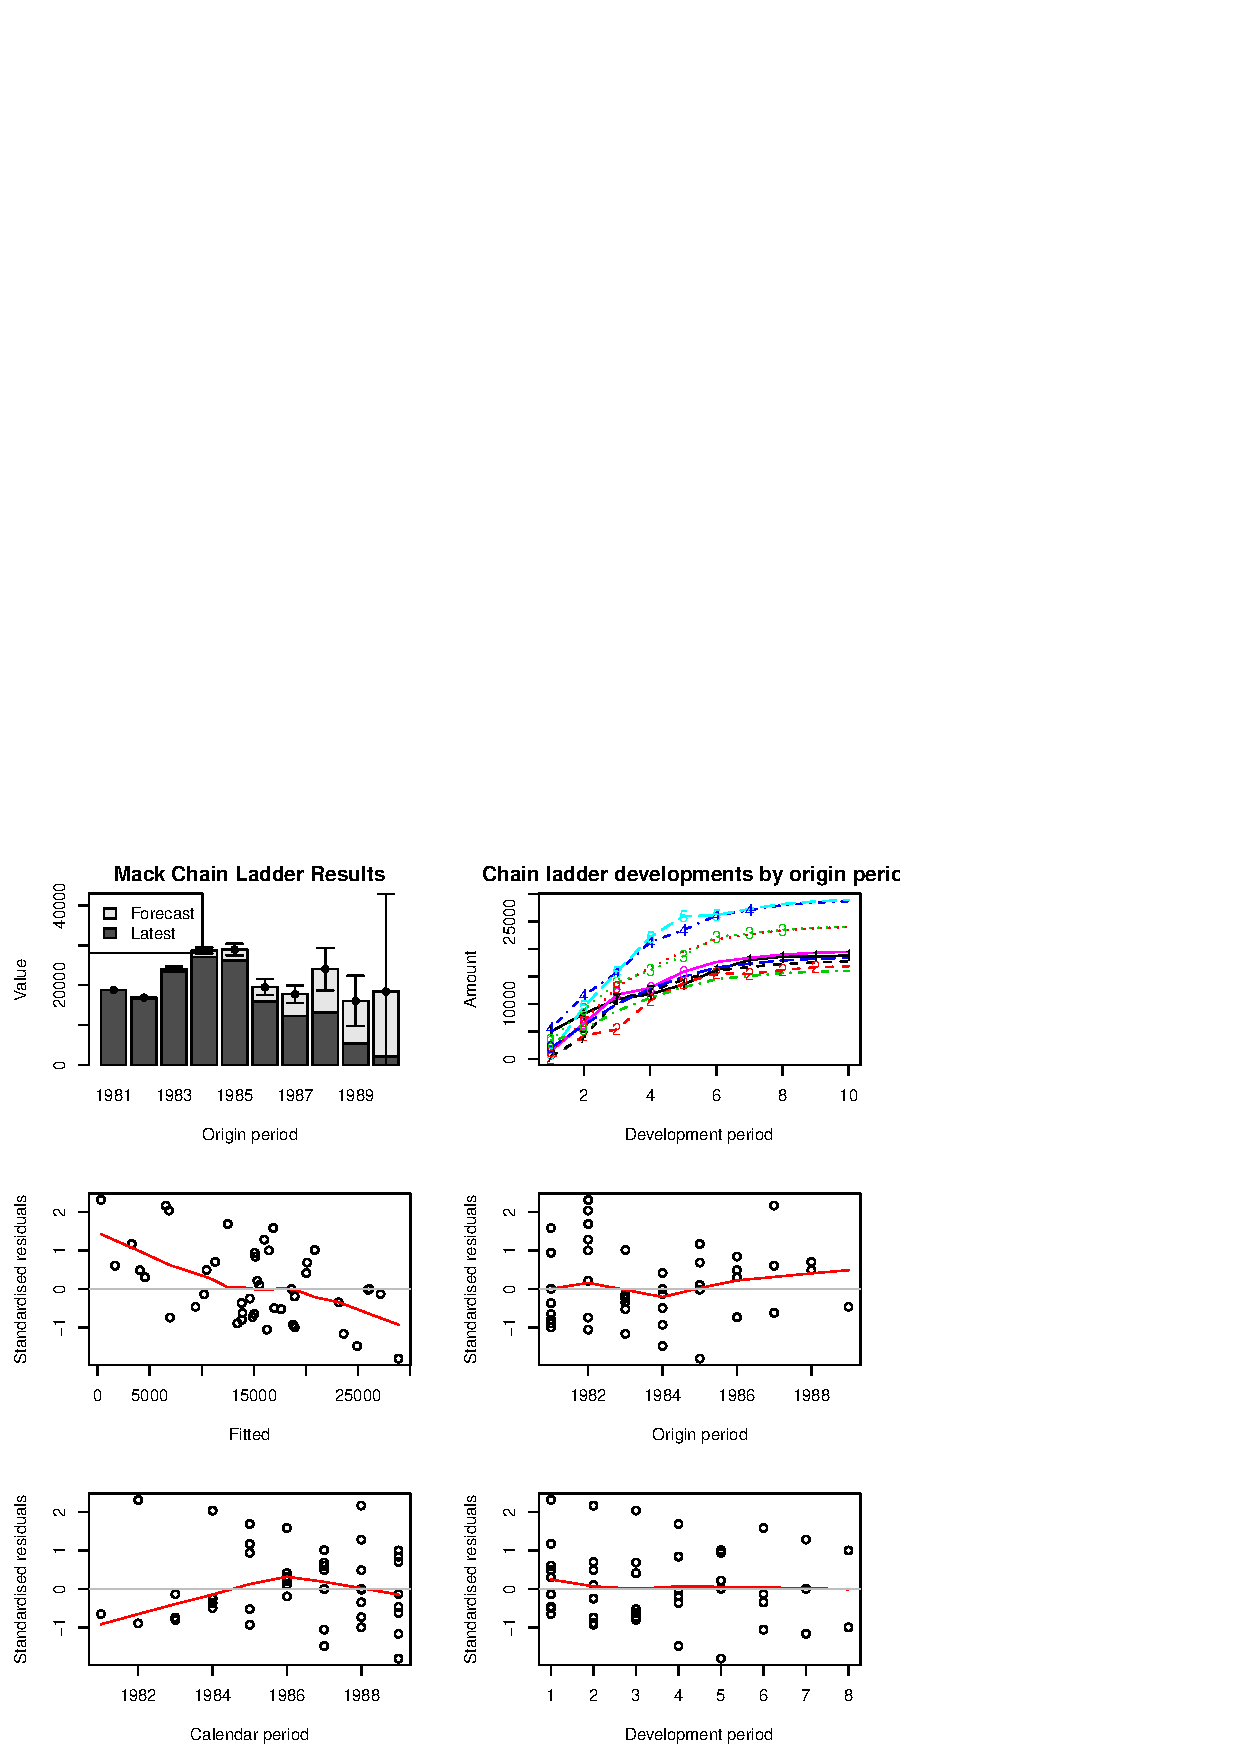
\includegraphics{ChainLadder-012}
    \caption{\texttt{plot(M)}}
  \end{center}
\end{figure}

The residual plots show the standardised residuals against fitted values, origin period, calendar period and development period.

All residual plots should show no pattern or direction for Mack's method to be applicable.

Pattern in any direction can be the result of trends and require further investigations.


\subsection{MunichChainLadder}
Munich-chain-ladder (MCL) is an extension of Mack?s method that reduces the gap between IBNR projections based on paid (P) and incurred (I) losses
Mack has to be applicable to both triangles
MCL adjusts the chain-ladder link-ratios depending if the momentary (P/I) ratio is above or below average
MCL uses the correlation of residuals between P vs. (I/P) and I vs. (P/I) chain-ladder link-ratio to estimate the correction factor
\begin{Schunk}
\begin{Sinput}
> Paid <- MCLpaid
> Incurred <- MCLincurred
> MackPaid = MackChainLadder(Paid)
> MackIncurred = MackChainLadder(Incurred)
> mean.pi <- apply(Paid/Incurred, 2, mean, na.rm = TRUE)
\end{Sinput}
\end{Schunk}
\begin{figure}[h]
  \begin{center}
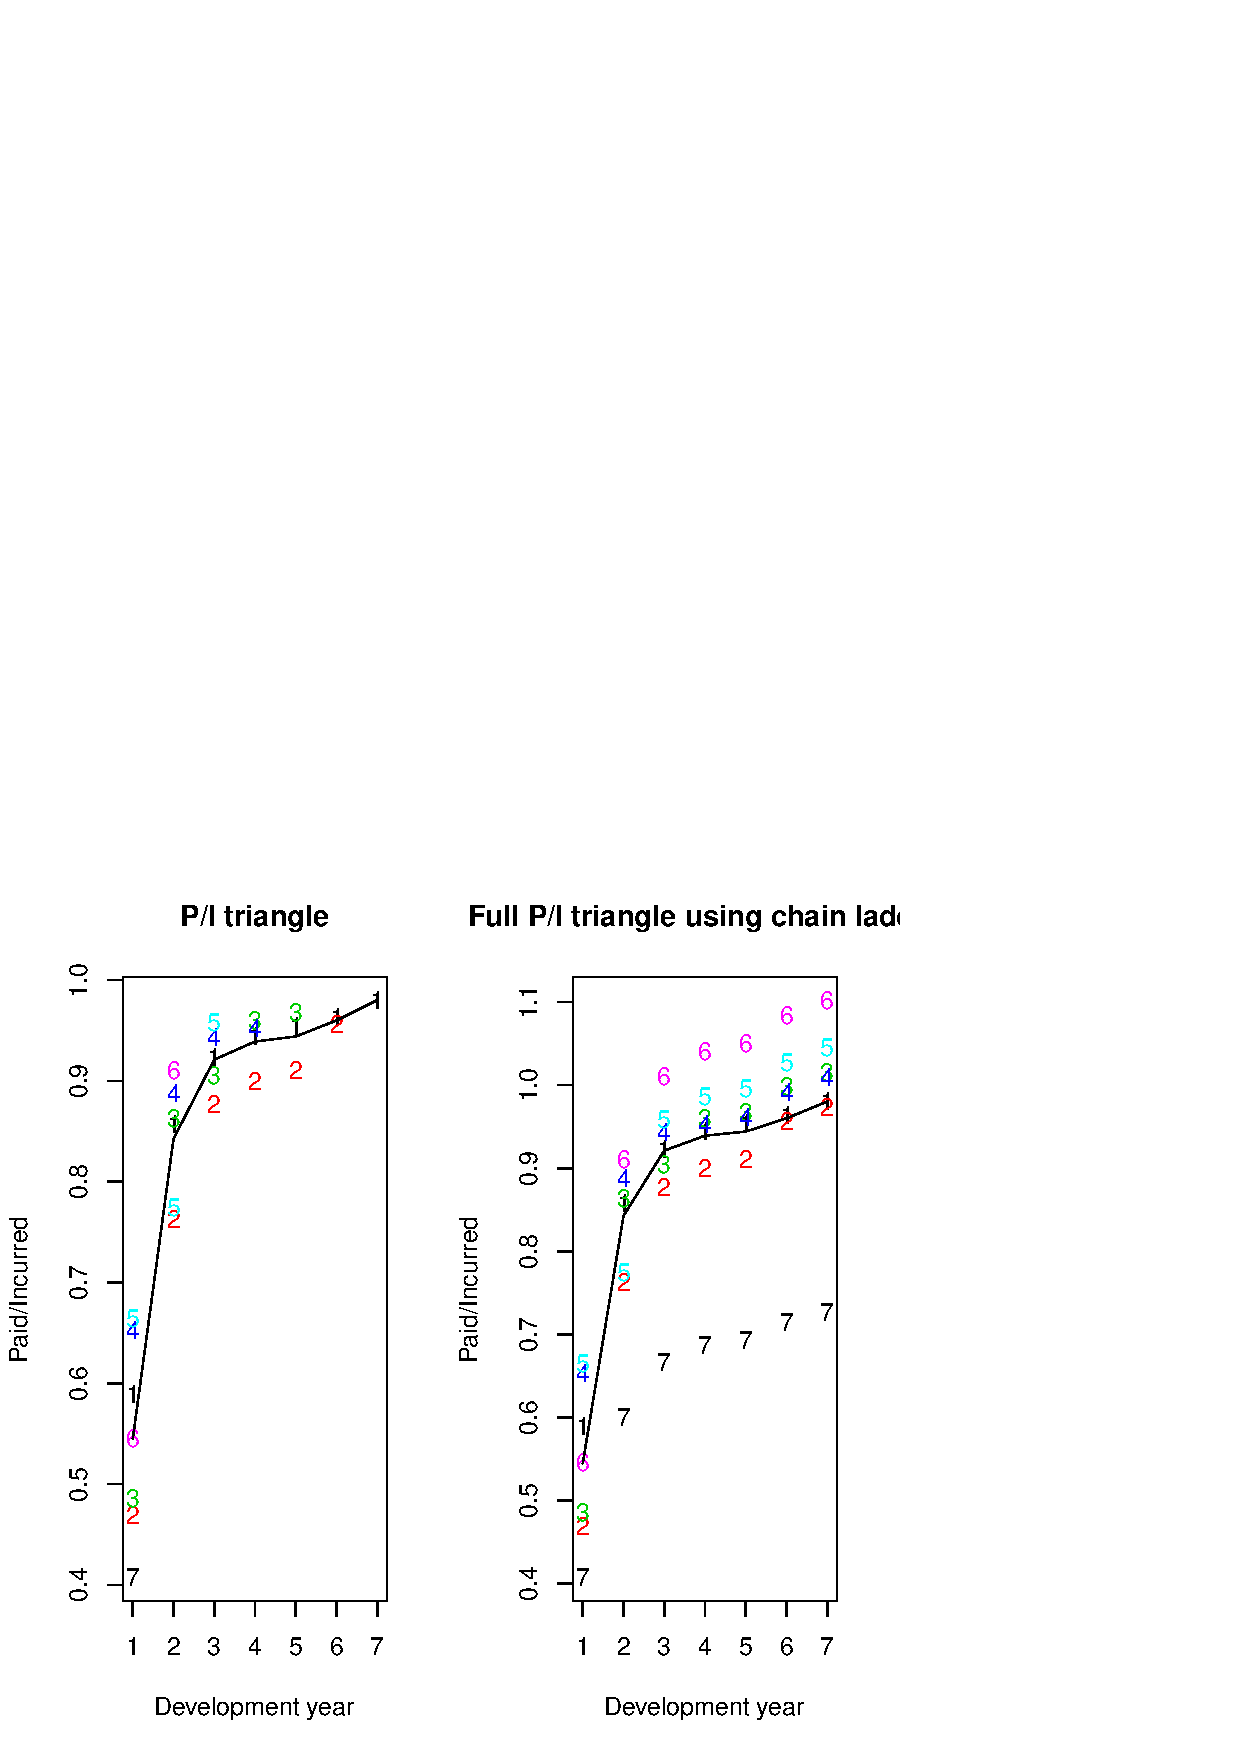
\includegraphics{ChainLadder-014}
    \caption{\texttt{plot(M)}}
  \end{center}
\end{figure}

Usage:
\texttt{
MunichChainLadder(Paid, Incurred,
      est.sigmaP = "log-linear",
      est.sigmaI = "log-linear",
      tailP=FALSE, tailI=FALSE)
}

Paid: cumulative paid claims triangle
Incurred: cumulative incurred claims triangle
est.sigmaP, est.sigmaI: Estimator for sigman-1
tailP, tailI: estimator for the tail
\begin{Schunk}
\begin{Sinput}
> MCL <- MunichChainLadder(Paid = MCLpaid, Incurred = MCLincurred, 
+     est.sigmaP = 0.1, est.sigmaI = 0.1)
> MCL
\end{Sinput}
\begin{Soutput}
MunichChainLadder(Paid = MCLpaid, Incurred = MCLincurred, est.sigmaP = 0.1, 
    est.sigmaI = 0.1)

  Latest Paid Latest Incurred Latest P/I Ratio Ult. Paid Ult. Incurred
1       2,131           2,174            0.980     2,131         2,174
2       2,348           2,454            0.957     2,383         2,444
3       4,494           4,644            0.968     4,597         4,629
4       5,850           6,142            0.952     6,119         6,176
5       4,648           4,852            0.958     4,937         4,950
6       4,010           4,406            0.910     4,656         4,665
7       2,044           5,022            0.407     7,549         7,650
  Ult. P/I Ratio
1          0.980
2          0.975
3          0.993
4          0.991
5          0.997
6          0.998
7          0.987

Totals
            Paid Incurred P/I Ratio
Latest:   25,525   29,694      0.86
Ultimate: 32,371   32,688      0.99
\end{Soutput}
\end{Schunk}
\begin{figure}[h]
  \begin{center}
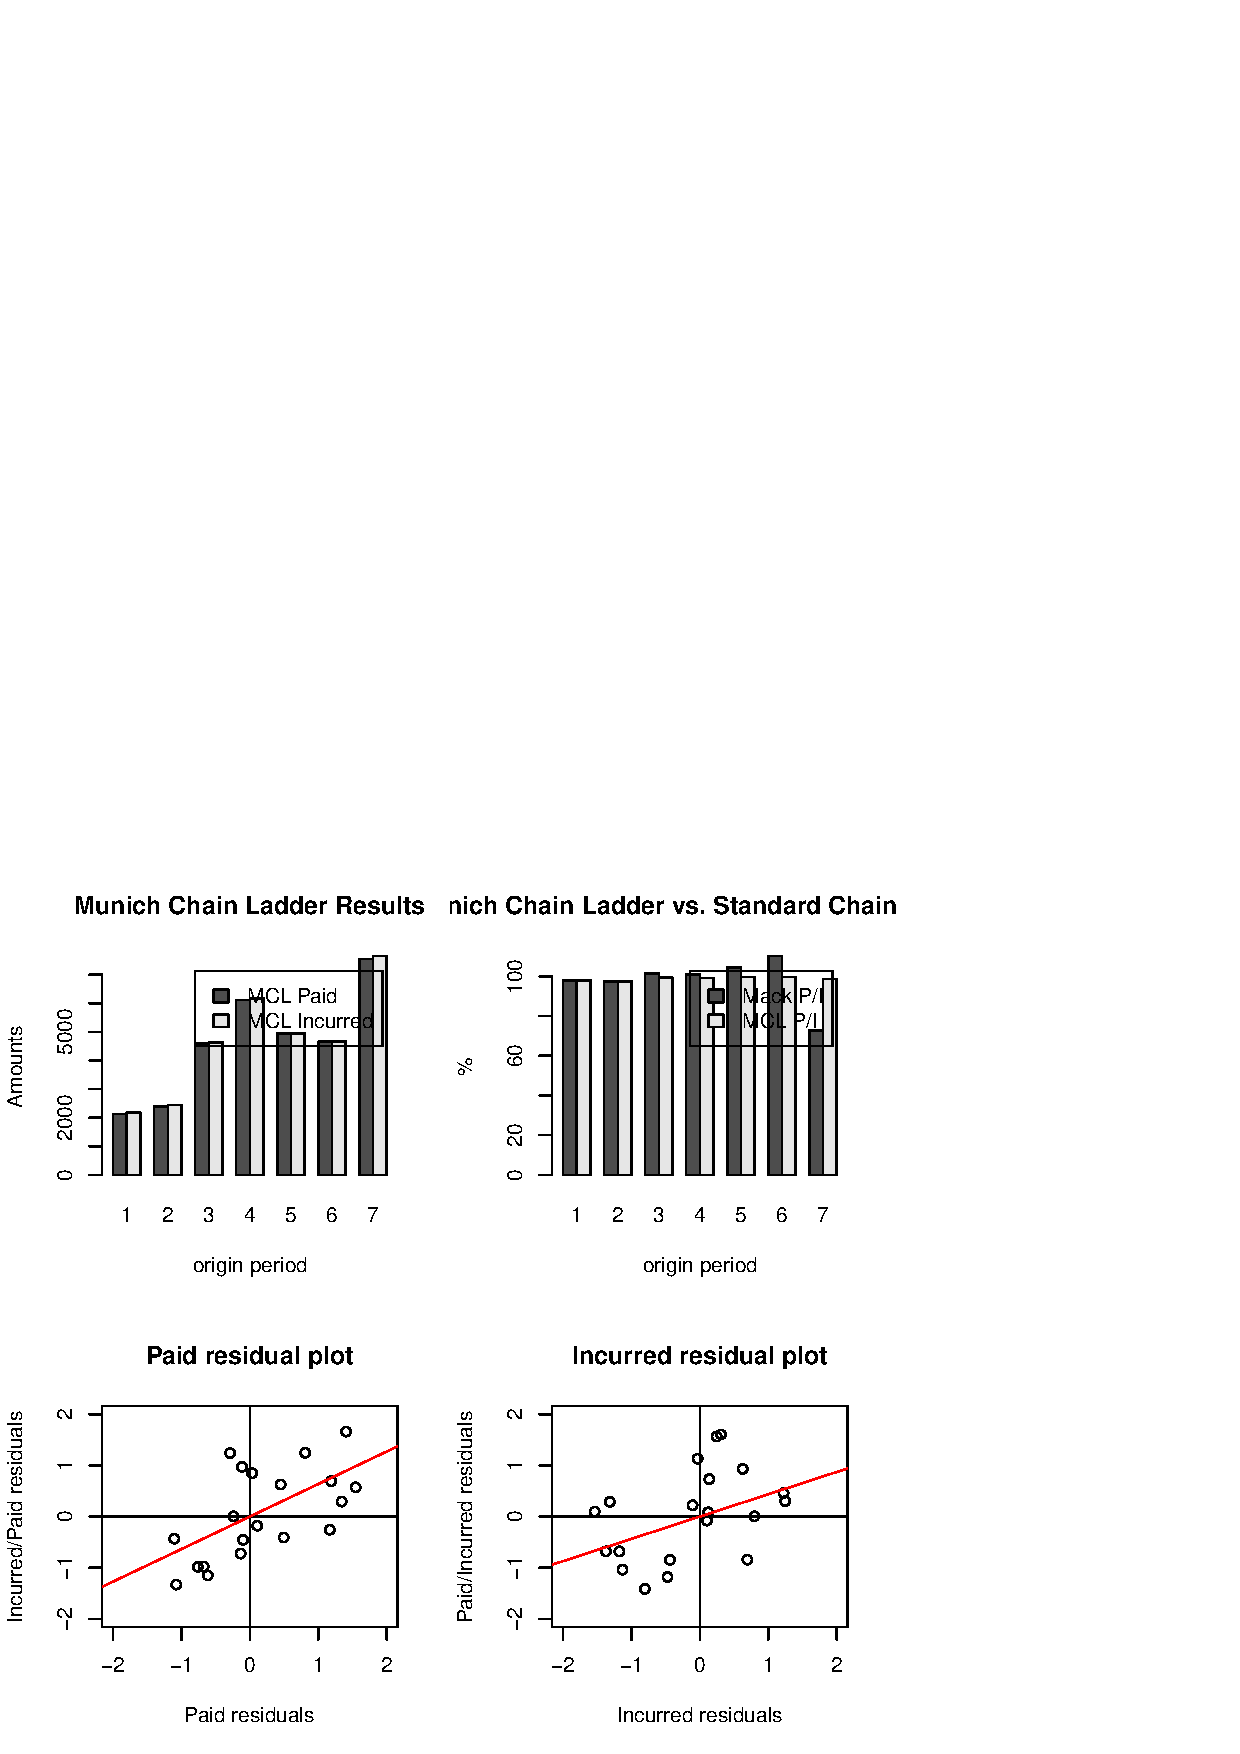
\includegraphics{ChainLadder-016}
    \caption{\texttt{plot(M)}}
  \end{center}
\end{figure}

MCL forecasts on P and I
Comparison of Ultimate P/I ratios of MCL and Mack
I/P link-ratio residuals against P link-ratio residuals
P/I link-ratio residuals against I link-ratios residuals

\subsection{BootChainLadder}

BootChainLadder uses a two-stage approach.
Calculate the scaled Pearson residuals and bootstrap R times to forecast future incremental claims payments via the standard chain-ladder method.
Simulate the process error with the bootstrap value as the mean and using an assumed process distribution.
The set of reserves obtained in this way forms the predictive distribution, from which summary statistics such as mean, prediction error or quantiles can be derived.

Usage: \texttt{
BootChainLadder(Triangle, R = 999,
    process.distr=c("gamma",
                    "od.pois"))
}

Triangle: cumulative claims triangle
R: Number of resampled bootstraps
process.distr: Assumed process distribution


\begin{Schunk}
\begin{Sinput}
> set.seed(1)
> B <- BootChainLadder(Triangle = RAA, R = 999, process.distr = "od.pois")
> B
\end{Sinput}
\begin{Soutput}
BootChainLadder(Triangle = RAA, R = 999, process.distr = "od.pois")

     Latest Mean Ultimate Mean IBNR SD IBNR IBNR 75% IBNR 95%
1981 18,834        18,834         0       0        0        0
1982 16,704        16,921       217     710      253    1,597
1983 23,466        24,108       642   1,340    1,074    3,205
1984 27,067        28,739     1,672   1,949    2,679    4,980
1985 26,180        29,077     2,897   2,467    4,149    7,298
1986 15,852        19,611     3,759   2,447    4,976    8,645
1987 12,314        17,724     5,410   3,157    7,214   11,232
1988 13,112        24,219    11,107   5,072   14,140   20,651
1989  5,395        16,119    10,724   6,052   14,094   21,817
1990  2,063        18,714    16,651  13,426   24,459   42,339

                 Totals
Latest:         160,987
Mean Ultimate:  214,066
Mean IBNR:       53,079
SD IBNR:         18,884
Total IBNR 75%:  64,788
Total IBNR 95%:  88,037
\end{Soutput}
\end{Schunk}

\begin{figure}[h]
  \begin{center}
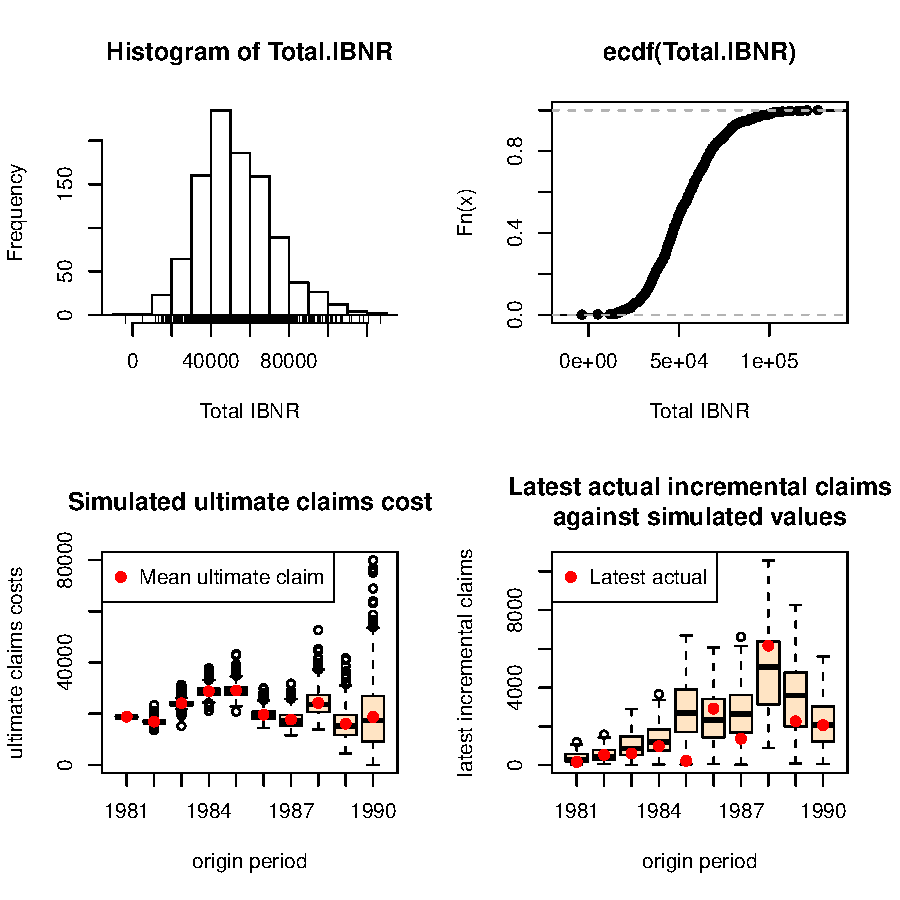
\includegraphics{ChainLadder-018}
    \caption{\texttt{plot(M)}}
  \end{center}
\end{figure}

Histogram of simulated total IBNR
Empirical distribution of total IBNR
Box-whisker plot of simulated ultimate claims cost by origin period
Test if latest actual incremental loss could come from simulated distribution of claims cost

\subsection{Generic Methods}

Mack-, Munich-, BootChainLadder
names: gives the individual elements back
summary: summary by origin and totals
print: nice formatted output
plot: plot overview of the results
MackChainLadder
residuals: chain-ladder residuals
BootChainLadder
mean: mean IBNR by origin and totals
quantile: gives quantiles of the simulation back

\section{R and databases}
Triangles are usually stored in databases
Triangles are stored in long tables
Use ODBC to connect to databases
Use SQL to interact with databases
Use R to transform tables into triangles
Apply ChainLadder function across many triangles in one statement
Write results back into database
\begin{figure}[h]
  \begin{center}
\includegraphics{Rdatabases}
    \caption{\texttt{plot(M)}}
  \end{center}
\end{figure}

\subsection{Create sample data in a table format}
Use example data sets to create a sample data table
\begin{Schunk}
\begin{Sinput}
> tri = list(RAA = RAA, Mortgage = Mortgage, GenIns = GenIns, ABC = ABC)
> longTriangle <- function(triangle) {
+     long <- expand.grid(origin = as.numeric(dimnames(triangle)$origin), 
+         dev = as.numeric(dimnames(triangle)$dev))
+     long$value <- as.vector(triangle)
+     return(na.omit(long))
+ }
> ltri <- lapply(tri, longTriangle)
> ltri <- lapply(names(ltri), function(x) data.frame(LOB = x, ltri[[x]]))
> triangleTable <- do.call("rbind", ltri)
\end{Sinput}
\end{Schunk}
\subsection{Write test data into database}
Example with MS Access 2003
See also documentation for RODBC

\begin{verbatim}
library(RODBC)
# Create a test database in c:/Temp (here MS Access 2003)
channel <- odbcConnectAccess(
"C:/Temp/ChainLadderTestData.mdb")
sqlSave(channel, triangleTable, "tblTestTriangles", rownames=FALSE)
odbcClose(channel)
}
\end{verbatim}

Access data via ODBC and SQL-statements
\begin{verbatim}
# From database
channel <- odbcConnectAccess(
  "C:/Temp/ChainLadderTestData.mdb")
myData <- sqlQuery(channel,
   "SELECT * FROM tblTestTriangles;")
odbcClose(channel)
}
\end{verbatim}

As an aside: Plot tables with lattice

Triangles stored in long tables are much easier to plot than triangles in cross-tab formats

 Plot long triangles
\begin{Schunk}
\begin{Sinput}
> library(lattice)
> P <- xyplot(value/1e+06 ~ dev | LOB, groups = origin, t = "l", 
+     data = myData, scales = "free")
\end{Sinput}
\end{Schunk}
\begin{figure}[h]
  \begin{center}
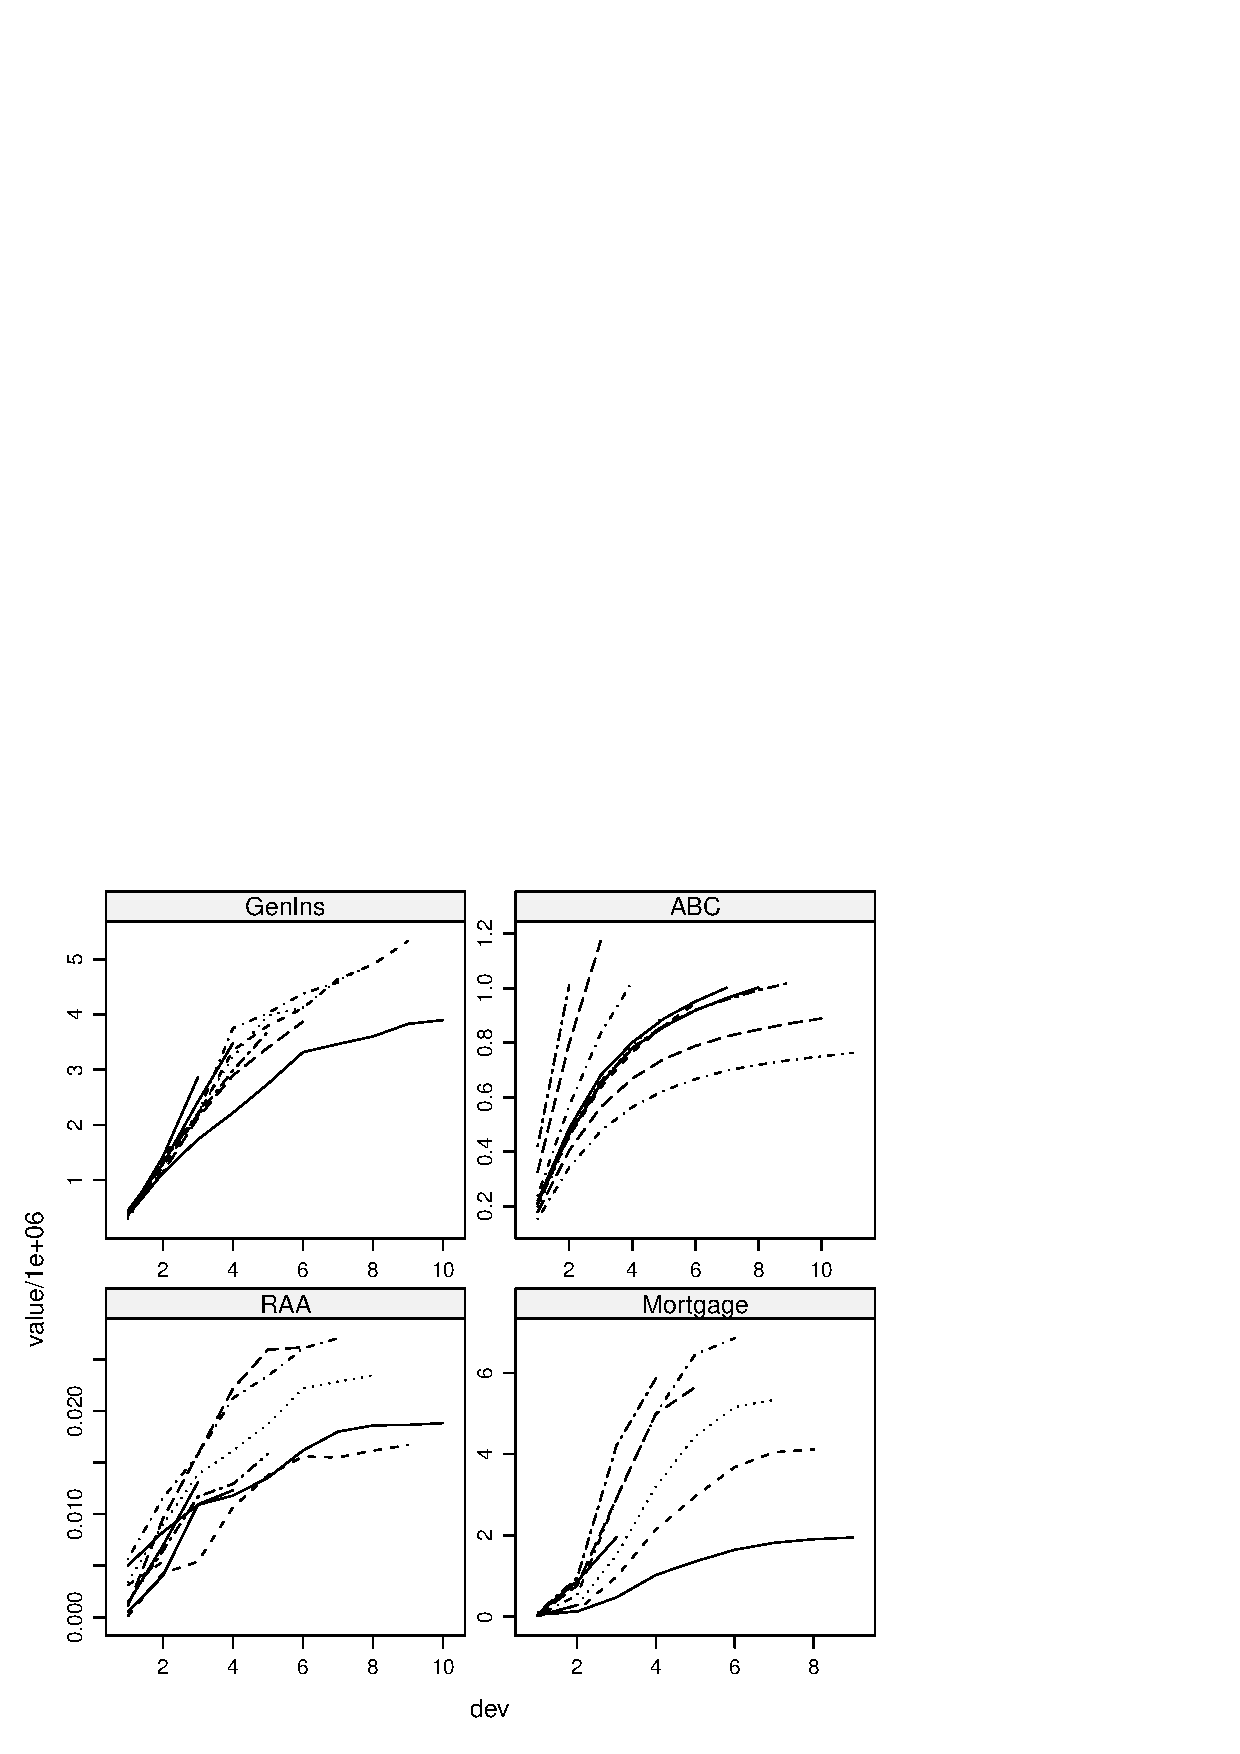
\includegraphics{ChainLadder-022}
    \caption{\texttt{plot(M)}}
  \end{center}
\end{figure}

\subsection{Transform tables into triangles}

We use the array function rather than reshape,    as its output is ready to be used by ChainLadder

\begin{Schunk}
\begin{Sinput}
> as.ArrayTriangle <- function(x) {
+     .names <- apply(x[, c("origin", "dev", "value")], 2, unique)
+     .namesOD <- .names[c("origin", "dev")]
+     .id <- paste(x$origin, x$dev, sep = ".")
+     .grid <- expand.grid(.namesOD)
+     .grid$id <- paste(.grid$origin, .grid$dev, sep = ".")
+     .grid$data <- x$value[match(.grid$id, .id)]
+     .data <- array(.grid$data, dim = unlist(lapply(.namesOD, 
+         length)), dimnames = .namesOD)
+     return(.data)
+ }
\end{Sinput}
\end{Schunk}

by function applies functions on sub sets of data
convert table for each LOB into a triangle
apply MackChainLadder for each triangle
Output is stored in a list
\begin{Schunk}
\begin{Sinput}
> myResults <- by(myData, list(LOB = myData$LOB), function(x) {
+     triangle <- as.ArrayTriangle(x)
+     M <- MackChainLadder(triangle, est.sigma = "Mack")
+     return(M)
+ })
> myResults
\end{Sinput}
\begin{Soutput}
LOB: RAA
MackChainLadder(Triangle = triangle, est.sigma = "Mack")

     Latest Dev.To.Date Ultimate   IBNR Mack.S.E CV(IBNR)
1981 18,834       1.000   18,834      0        0      NaN
1982 16,704       0.991   16,858    154      206    1.339
1983 23,466       0.974   24,083    617      623    1.010
1984 27,067       0.943   28,703  1,636      747    0.457
1985 26,180       0.905   28,927  2,747    1,469    0.535
1986 15,852       0.813   19,501  3,649    2,002    0.549
1987 12,314       0.694   17,749  5,435    2,209    0.406
1988 13,112       0.546   24,019 10,907    5,358    0.491
1989  5,395       0.336   16,045 10,650    6,333    0.595
1990  2,063       0.112   18,402 16,339   24,566    1.503

               Totals
Latest:    160,987.00
Ultimate:  213,122.23
IBNR:       52,135.23
Mack S.E.:  26,909.01
CV(IBNR):        0.52
------------------------------------------------------------ 
LOB: Mortgage
MackChainLadder(Triangle = triangle, est.sigma = "Mack")

     Latest Dev.To.Date  Ultimate      IBNR  Mack.S.E CV(IBNR)
1 1,950,105      1.0000 1,950,105         0         0      NaN
2 4,115,760      0.9778 4,209,118    93,358    60,883    0.652
3 5,342,585      0.9527 5,607,658   265,073   139,670    0.527
4 6,853,904      0.8915 7,688,163   834,259   319,020    0.382
5 5,648,563      0.7828 7,216,272 1,567,709   596,210    0.380
6 5,866,482      0.6135 9,562,602 3,696,120 1,037,862    0.281
7 1,954,797      0.3592 5,442,091 3,487,294 1,298,251    0.372
8   284,441      0.0878 3,240,567 2,956,126 1,806,032    0.611
9    13,121      0.0079 1,659,913 1,646,792 2,182,258    1.325

                  Totals
Latest:    32,029,758.00
Ultimate:  46,576,488.14
IBNR:      14,546,730.14
Mack S.E.:  3,728,870.24
CV(IBNR):           0.26
------------------------------------------------------------ 
LOB: GenIns
MackChainLadder(Triangle = triangle, est.sigma = "Mack")

      Latest Dev.To.Date  Ultimate      IBNR  Mack.S.E CV(IBNR)
1  3,901,463      1.0000 3,901,463         0         0      NaN
2  5,339,085      0.9826 5,433,719    94,634    75,535    0.798
3  4,909,315      0.9127 5,378,826   469,511   121,699    0.259
4  4,588,268      0.8661 5,297,906   709,638   133,549    0.188
5  3,873,311      0.7973 4,858,200   984,889   261,406    0.265
6  3,691,712      0.7223 5,111,171 1,419,459   411,010    0.290
7  3,483,130      0.6153 5,660,771 2,177,641   558,317    0.256
8  2,864,498      0.4222 6,784,799 3,920,301   875,328    0.223
9  1,363,294      0.2416 5,642,266 4,278,972   971,258    0.227
10   344,014      0.0692 4,969,825 4,625,811 1,363,155    0.295

                  Totals
Latest:    34,358,090.00
Ultimate:  53,038,945.61
IBNR:      18,680,855.61
Mack S.E.:  2,447,094.86
CV(IBNR):           0.13
------------------------------------------------------------ 
LOB: ABC
MackChainLadder(Triangle = triangle, est.sigma = "Mack")

        Latest Dev.To.Date  Ultimate      IBNR Mack.S.E CV(IBNR)
1977   762,544       1.000   762,544         0        0      NaN
1978   889,022       0.984   903,477    14,455      285   0.0197
1979 1,019,932       0.965 1,057,440    37,508      923   0.0246
1980 1,002,134       0.940 1,066,050    63,916    2,758   0.0431
1981 1,002,194       0.909 1,102,586   100,392    5,715   0.0569
1982   944,614       0.868 1,088,663   144,049    7,613   0.0529
1983   895,700       0.809 1,107,375   211,675   14,854   0.0702
1984 1,024,228       0.726 1,409,929   385,701   22,419   0.0581
1985 1,173,448       0.605 1,938,303   764,855   37,293   0.0488
1986 1,011,178       0.426 2,373,610 1,362,432   62,244   0.0457
1987   496,200       0.185 2,688,977 2,192,777  107,919   0.0492

                  Totals
Latest:    10,221,194.00
Ultimate:  15,498,954.36
IBNR:       5,277,760.36
Mack S.E.:    152,283.14
CV(IBNR):           0.03
\end{Soutput}
\end{Schunk}
Combine results in tables

Use lapply to access MackChainLadder output
Access origin year and total results separately

\begin{Schunk}
\begin{Sinput}
> OriginResults <- lapply(lapply(myResults, summary), "[[", "ByOrigin")
> OriginResults <- lapply(names(OriginResults), function(x) data.frame(LOB = x, 
+     OriginResults[[x]]))
> OriginResultsTable <- do.call("rbind", OriginResults)
> OriginResultsTable
\end{Sinput}
\begin{Soutput}
           LOB  Latest Dev.To.Date   Ultimate         IBNR     Mack.S.E
1981       RAA   18834 1.000000000   18834.00       0.0000       0.0000
1982       RAA   16704 0.990867580   16857.95     153.9539     206.2201
1983       RAA   23466 0.974365261   24083.37     617.3709     623.3767
1984       RAA   27067 0.942997803   28703.14    1636.1422     747.1752
1985       RAA   26180 0.905045066   28926.74    2746.7363    1469.4571
1986       RAA   15852 0.812877090   19501.10    3649.1032    2001.8569
1987       RAA   12314 0.693773738   17749.30    5435.3026    2209.2421
1988       RAA   13112 0.545896786   24019.19   10907.1925    5357.8693
1989       RAA    5395 0.336242153   16044.98   10649.9841    6333.1659
1990       RAA    2063 0.112104684   18402.44   16339.4425   24566.2879
1     Mortgage 1950105 1.000000000 1950105.00       0.0000       0.0000
2     Mortgage 4115760 0.977820169 4209117.52   93357.5166   60883.4330
3     Mortgage 5342585 0.952730151 5607658.15  265073.1526  139670.2698
4     Mortgage 6853904 0.891487837 7688163.22  834259.2176  319019.6484
5     Mortgage 5648563 0.782753618 7216271.97 1567708.9746  596210.2865
6     Mortgage 5866482 0.613481768 9562602.04 3696120.0355 1037861.7566
7     Mortgage 1954797 0.359199633 5442090.75 3487293.7541 1298251.3107
8     Mortgage  284441 0.087775080 3240566.68 2956125.6789 1806031.7003
9     Mortgage   13121 0.007904632 1659912.81 1646791.8146 2182258.4258
11      GenIns 3901463 1.000000000 3901463.00       0.0000       0.0000
21      GenIns 5339085 0.982583969 5433718.81   94633.8145   75535.0408
31      GenIns 4909315 0.912711200 5378826.29  469511.2901  121698.5616
41      GenIns 4588268 0.866053145 5297905.82  709637.8208  133548.8530
51      GenIns 3873311 0.797272917 4858199.64  984888.6390  261406.4493
61      GenIns 3691712 0.722282950 5111171.46 1419459.4577  411009.7039
71      GenIns 3483130 0.615310217 5660770.62 2177640.6201  558316.8581
81      GenIns 2864498 0.422193494 6784799.01 3920301.0120  875327.5119
91      GenIns 1363294 0.241621706 5642266.26 4278972.2633  971257.8065
10      GenIns  344014 0.069220550 4969824.69 4625810.6944 1363154.9117
1977       ABC  762544 1.000000000  762544.00       0.0000       0.0000
1978       ABC  889022 0.984000923  903476.79   14454.7946     285.2779
1979       ABC 1019932 0.964529378 1057440.06   37508.0570     922.8391
1980       ABC 1002134 0.940044355 1066049.70   63915.6970    2757.5189
19811      ABC 1002194 0.908948519 1102586.10  100392.0974    5715.0360
19821      ABC  944614 0.867682368 1088663.36  144049.3581    7613.2481
19831      ABC  895700 0.808850045 1107374.61  211674.6058   14854.3038
19841      ABC 1024228 0.726439364 1409929.10  385701.1013   22418.9809
19851      ABC 1173448 0.605399556 1938303.37  764855.3698   37293.3620
19861      ABC 1011178 0.426008396 2373610.50 1362432.4958   62243.5590
19871      ABC  496200 0.184531158 2688976.78 2192776.7808  107918.9156
        CV.IBNR.
1981         NaN
1982  1.33949212
1983  1.00972794
1984  0.45666889
1985  0.53498296
1986  0.54858874
1987  0.40646166
1988  0.49122350
1989  0.59466435
1990  1.50349609
1            NaN
2     0.65215352
3     0.52691217
4     0.38239871
5     0.38030674
6     0.28079763
7     0.37228046
8     0.61094551
9     1.32515744
11           NaN
21    0.79818235
31    0.25920263
41    0.18819298
51    0.26541727
61    0.28955368
71    0.25638613
81    0.22328069
91    0.22698390
10    0.29468454
1977         NaN
1978  0.01973587
1979  0.02460376
1980  0.04314306
19811 0.05692715
19821 0.05285166
19831 0.07017518
19841 0.05812527
19851 0.04875871
19861 0.04568561
19871 0.04921564
\end{Soutput}
\begin{Sinput}
> TotalResults <- lapply(lapply(lapply(myResults, summary), "[[", 
+     "Totals"), t)
> TotalResults <- lapply(names(TotalResults), function(x) data.frame(LOB = x, 
+     TotalResults[[x]]))
> TotalResultsTable <- do.call("rbind", TotalResults)
> TotalResultsTable
\end{Sinput}
\begin{Soutput}
             LOB  Latest.  Ultimate.       IBNR. Mack.S.E..  CV.IBNR..
Totals       RAA   160987   213122.2    52135.23   26909.01 0.51613874
Totals1 Mortgage 32029758 46576488.1 14546730.14 3728870.24 0.25633735
Totals2   GenIns 34358090 53038945.6 18680855.61 2447094.86 0.13099480
Totals3      ABC 10221194 15498954.4  5277760.36  152283.14 0.02885374
\end{Soutput}
\end{Schunk}

Write results back into new tables of the database via QDBC and sqlSave

\begin{verbatim}
channel <- odbcConnectAccess("C:/Temp/ChainLadderTestData.mdb")
sqlSave(channel, OriginResultsTable, "myOriginResults",
rownames=FALSE)
sqlSave(channel, TotalResultsTable, "myTotalResults",
rownames=FALSE)
odbcClose(channel)
\end{verbatim}
\subsection{Database summary}
Use R to query DB
Transform table to triangles
Apply ChainLadder function across all triangles
Summaries results
Save results in DB
\section{R and MS Office interfaces}
\subsection{Windows meta-file}
Windows meta-file (WMF, or EMF (Enhanced meta-file) is a vector graphic format
High quality, but editable format for MS Office
Create WMF-files in R with win.metafile()

\begin{verbatim}
win.metafile(file="C:/Temp/Testplot.wmf")
plot(sin(seq(0,round(2*pi,2),0.01)))
dev.off()
\end{verbatim}

\subsection{Clipboard to exchange data}
Copy and paste from R to and from Excel

\subsubsection{R $\to$ Excel}

\begin{verbatim}
mydf=data.frame(x=1:10, y=letters[1:10])
write.table(mydf, file="clipboard", sep="\t", row.names=FALSE)
\end{verbatim}
\subsubsection{Excel $\to$ R}
\begin{verbatim}
read.table(file= "clipboard", sep="\t")
\end{verbatim}

\subsection{RExcel - Using R from within Excel}
RExcel Add-in allows to use R functions from Excel, see: http://sunsite.univie.ac.at/rcom/

There are at least three different ways of using R from within Excel

Scratchpad mode
Writing R Code directly in an Excel worksheet and transferring scalar, vector, and matrix variables between R and Excel
Macro mode
Writing macros using VBA and the macros supplied by RExcel, attaching the macros to menu items or toolbar items
Worksheet functions
R can be called directly in functions in worksheet cells

RExcel allows to use R functions within Excel
Package comes with example file
R function can be embedded and are interactive
Use R graphics

\subsection{Using the COM server (VBA Example)}

StatConnector allows to use R within MS Office VBA
Add reference to StatConnectorSrv 1.1 Type Library
\begin{verbatim}
Sub FirstR()
Dim nrandom As Integer, x As Double
nrandom = 100
Set StaR = New StatConnector
StaR.Init ("R")

With StaR
	.SetSymbol "n", nrandom
	.EvaluateNoReturn ("x <- rnorm(n)")
	.EvaluateNoReturn ("pdf(file='c:/Temp/Testplot.pdf')")
	.EvaluateNoReturn ("hist(x)")
	.EvaluateNoReturn ("dev.off()")
	x = .Evaluate("summary(x)")
End With

Debug.Print "Min.  1st Qu.  Median  Mean  3rd Qu.  Max. "
Debug.Print x(0), x(1), x(2), x(3), x(4), x(5)

End Sub
\end{verbatim}


\subsection{rcom: Control MS Office from R}
Using the rcom R-package you can write output from R into MS Office application
Example: Create PowerPoint slide with MackChainLadder output

\begin{verbatim}
library(ChainLadder)
R <- MackChainLadder(RAA)
myfile=tempfile()
win.metafile(file=myfile)
plot(R)
dev.off()
#
library(rcom)
ppt<-comCreateObject("Powerpoint.Application")
comSetProperty(ppt,"Visible",TRUE)
myPresColl<-comGetProperty(ppt,"Presentations")
myPres<-comInvoke(myPresColl,"Add")
mySlides<-comGetProperty(myPres,"Slides")
mySlide<-comInvoke(mySlides,"Add",1,12)
myShapes<-comGetProperty(mySlide,"Shapes")
myPicture<-comInvoke(myShapes,"AddPicture",myfile,0,1,100,10)
\end{verbatim}

\section{More help}

See examples on project web page
Read documentation on CRAN: http://cran.r-project.org/web/packages/ChainLadder/ChainLadder.pdf
Read help pages in R:

\begin{verbatim}
?MackChainLadder
?MunichChainLadder
?BootChainLadder
\end{verbatim}
Follow examples in R:

\begin{verbatim}
example(MackChainLadder)
example(MunichChainLadder)
example(BootChainLadder)
\end{verbatim}

See also the \pkg{actuar}~\citep{actuar} and R introduction for actuaries~\citep{DeSilva}

\section{Conclusion}

R is ideal for reserving
Built-in functions for statistical modelling
Powerful language for data manipulations
Fantastic graphical capabilities for analysis and presentation
Easy to set-up connections to databases (ODBC)
RExcel add-in allows to share R functions with colleagues without R knowledge
rcom allows to control MS Office from R
Effective knowledge transfer - plain text files

\begin{verbatim}
library(rgl) #provides interactive 3d plotting functions
MCL=MackChainLadder(GenIns/1e6)
FT <- MCL$FullTriangle
FTpSE <- FT+MCL$Mack.S.E
FTpSE[which(MCL$Mack.S.E==0, arr.ind=TRUE)] <- NA
FTmSE <- FT-MCL$Mack.S.E
FTmSE[which(MCL$Mack.S.E==0, arr.ind=TRUE)] <- NA
zr <- round(FT/FT[1,10]*100)
zlim <- range(zr, na.rm=TRUE)
zlen <- zlim[2] - zlim[1] + 1
colorlut <- terrain.colors(zlen) # height color lookup table
cols <- colorlut[ zr -zlim[1]+1 ] # assign colors to heights for each point
x <- as.numeric(dimnames(FT)$origin)
y <- as.numeric(dimnames(FT)$dev)
persp3d(x, y=y,
        z=(FT), col=cols, xlab="origin", ylab="dev", zlab="loss",back="lines")
mSE <- data.frame(as.table(FTmSE))
points3d(xyz.coords(x=as.numeric(as.character(mSE$origin)),
    y=as.numeric(as.character(mSE$dev)),z=mSE$Freq), size=2)
pSE <- data.frame(as.table(FTpSE))
points3d(xyz.coords(x=as.numeric(as.character(pSE$origin)),
    y=as.numeric(as.character(pSE$dev)),z=pSE$Freq), size=2)

\end{verbatim}

\begin{figure}[h]
  \begin{center}
\includegraphics{Fancy3d}
    \caption{\texttt{plot(M)}}
  \end{center}
\end{figure}
\pagebreak

Reserves cover IBNR (Incurred But Not
Reported) claims Reserves are usually estimated based on
historical claims payment/reporting patterns  In the past a point estimator for the reserves
was sufficient New regulatory requirements ($\to$ Solvency II)
foster stochastic methods
R is a programming environment for data analysis and graphics.
R can be regarded as an implementation of
the S language which was developed at Bell Laboratories by Rick Becker,
John Chambers and Allan Wilks, and also forms the basis of the
S-Plus systems~\cite{splus}.
The R project was started by Robert Gentleman and Ross Ihaka of the Statistics
Department of the University of Auckland in 1995~\cite{IhakaGentelman1996}.
It has quickly gained a widespread audience. It is currently maintained by
the R core-development team under the GNU General Public License
(GPL)~\cite{GNU}.
The R project web page
%\begin{center}
\url{http://www.r-project.org}
%\end{center}


\section{The \pkg{ChainLadder} package}
\begin{Schunk}
\begin{Sinput}
> library(ChainLadder)
\end{Sinput}
\end{Schunk}

\subsection{Mack Chain Ladder}
\begin{Schunk}
\begin{Sinput}
> data(RAA)
> RAA
\end{Sinput}
\begin{Soutput}
        1     2     3     4     5     6     7     8     9    10
1981 5012  8269 10907 11805 13539 16181 18009 18608 18662 18834
1982  106  4285  5396 10666 13782 15599 15496 16169 16704    NA
1983 3410  8992 13873 16141 18735 22214 22863 23466    NA    NA
1984 5655 11555 15766 21266 23425 26083 27067    NA    NA    NA
1985 1092  9565 15836 22169 25955 26180    NA    NA    NA    NA
1986 1513  6445 11702 12935 15852    NA    NA    NA    NA    NA
1987  557  4020 10946 12314    NA    NA    NA    NA    NA    NA
1988 1351  6947 13112    NA    NA    NA    NA    NA    NA    NA
1989 3133  5395    NA    NA    NA    NA    NA    NA    NA    NA
1990 2063    NA    NA    NA    NA    NA    NA    NA    NA    NA
\end{Soutput}
\begin{Sinput}
> M = MackChainLadder(RAA)
> M
\end{Sinput}
\begin{Soutput}
MackChainLadder(Triangle = RAA)

     Latest Dev.To.Date Ultimate   IBNR Mack.S.E CV(IBNR)
1981 18,834       1.000   18,834      0        0      NaN
1982 16,704       0.991   16,858    154      143    0.928
1983 23,466       0.974   24,083    617      592    0.959
1984 27,067       0.943   28,703  1,636      713    0.436
1985 26,180       0.905   28,927  2,747    1,452    0.529
1986 15,852       0.813   19,501  3,649    1,995    0.547
1987 12,314       0.694   17,749  5,435    2,204    0.405
1988 13,112       0.546   24,019 10,907    5,354    0.491
1989  5,395       0.336   16,045 10,650    6,332    0.595
1990  2,063       0.112   18,402 16,339   24,566    1.503

               Totals
Latest:    160,987.00
Ultimate:  213,122.23
IBNR:       52,135.23
Mack S.E.:  26,880.74
CV(IBNR):        0.52
\end{Soutput}
\end{Schunk}





\bibliography{reserving}

\end{document}


